\Chapter{Review of the literature}{Part II: Operations research}
\label{cha:rol.mcda}

\begin{summary}
In this chapter, we briefly present the basics of multi-objective optimization and multi-criteria decision aid, in order to justify our choice to use such a paradigm. We will explain in what kind of context a multi-criteria approach can be used and present some classical methods of the field.
\end{summary}

\section{Introduction}
\label{sec:rol2.intro}
In this chapter, we will briefly present the basics of multi-objective optimization and multi-criteria decision aid, in order to justify our choice to use such a paradigm. As stated in Chapter \ref{cha:rol.icdesign}, the 3D integration can offer new perspectives but designing 3D-SICs includes two major distinctive features: multiple criteria and a huge number of possible solutions. When facing such problems, two main approches exist: the uni-criterion paradigm and the multi-criteria paradigm. For optimization problems, these paradigm will refer to the terminology mono-\emph{objective}/multi-\emph{objective} optimization while for decision aid, the terminology uni-\emph{criterion}/multi-\emph{criteria} will be used.

In the following, we will briefly describe each paradigm, showing some of the main approaches alongside illustrative examples. We will first present the uni-criterion methodology, show why it can be limited in our contect and explain why a multi-criteria paradigm can be more suitable.

\section{The uni-criterion paradigm}
\label{sec:rol2.unicrit_paradigm}

\subsection{Problem formulation}
An optimization problem can be formulated, without loss of generality, as \cite{BraMar2002}
\begin{equation}
\label{eqn:optiprob}
\begin{gathered}
\min f(x)\\
x \in A
\end{gathered}
\end{equation}
where $f$ is a real-valued function evaluating the solutions denoted $x$, and $A$ is the set of solutions, $f$ is also called the \emph{criterion} on which $x$ is evaluated. A criterion can therefore be defined as follows:

\begin{definition}[Criterion]
A criterion is a way to evaluate and compare potential solutions. These are evaluated according to a specific point of view, which then results in performance levels.
\end{definition}

Let us note that the equation \ref{eqn:optiprob} expresses a \emph{minimization} problem. A \emph{maximization} problem can be seen as a minimization problem with the identity
\begin{equation}
\max_{x \in A} f(x) = - \min_{x \in A} (-f(x))
\end{equation}
so that there is no loss of generality by using only \emph{minimization} formulation.

In order to give a more precise idea of what an optimization problem is, we will describe in the next section some typical examples taken from the reference book \cite{talbi09, BraMar2002}.

\subsection{Examples of typical optimization problems}
\subsubsection{Linear programming}
Linear programming (LP) is a problem formulation where the aim is to optimize a linear function, subject to linear inequality constraints. This can be formulated as follows:
\begin{equation}
\min \mathbf{c}^\intercal\mathbf{x}
\end{equation}
subject to
\begin{equation*}
\begin{gathered}
A\mathbf{x} \leq \mathbf{b}\\
\mathbf{x} \geq \mathbf{0}
\end{gathered}
\end{equation*}
where $\mathbf{x}$ is a vector of continuous, integer or boolean variables to be determined, $\mathbf{c}$ and $\mathbf{b}$ are vectors of coefficients, $A$ is a matrix of coefficients.

Efficient exact methods for solving LP problem exist such as, among the most knowns, the simplex algorithm \cite{dantzig51} or the interior point method \cite{Karmarkar84}.

\begin{example}[Linear programming]
A given company produces two electronic boards $Board_1$ and $Board_2$ based on two kinds of memories $M_1$ and $M_2$. The objective consists in finding the most profitable product mix, given the availability of each memory $M_1$ and $M_2$, and the amount of memory used as well as the profit per board, as shown in Table \ref{tab:ex_lp}. The decision variables are $x_1$ and $x_2$ that represent respectively the amount of $Board_1$ and $Board_2$ produced. The objective is to maximize the profit.\\
The problem can be formulated as an LP:
\begin{equation}
\text{max profit } = 5x_1 + 4x_2
\end{equation}
subject to the constraints
\begin{eqnarray*}
192x_1 + 128 x_2 &\leq& 1024\\
32x_1 + 64_x2 &\leq& 192\\
x_1, x_2 &\geq& 0
\end{eqnarray*}
\end{example}

\begin{table}[h!]
\begin{center}
\caption{Data associated with the LP problem}
\begin{tabular}{|l|c|c|c|}
\hline
& Usage for $Board_1$ & Usage for $Board_2$ & Availability\\
\hline
$M_1$ & 192 & 128 & 1024 \\
$M_2$ & 32 & 64 & 192 \\
Profit per unit & \euro 5 & \euro 4 & \\
\hline
\end{tabular}
\label{tab:ex_lp}
\end{center}
\end{table}

When the variables are restricted to integers, the problems are solved with integer linear programming (ILP):
\begin{equation}
\min \mathbf{c}^\intercal\mathbf{x}
\end{equation}
subject to
\begin{equation*}
\begin{gathered}
A\mathbf{x} \leq \mathbf{b}\\
%\mathbf{x} \geq \mathbf{0}\\
\mathbf{x} \in \mathbb{N}
\end{gathered}
\end{equation*}
where $\mathbf{c}$ and $\mathbf{b}$ are vectors and $A$ is a matrix of coefficients.

When the set of decision variables contains both discrete and continuous variables, the problem refers to \textbf{mixed integer programs} (MILP).

Other particular ILP problems which deals with variables that are restricted to be either 0 or 1 are called \textbf{0-1 linear programming}.

\begin{example}[Travelling salesman problem (TSP) \cite{talbi09}]
This is one of the most known optimization problem. It can be formulated as follows: given $n$ cities and the distance between each pair of cities, we have to find the shortest tour that visits each city once and returns to the origin city. This problem can be formulated as an ILP problem.\\
Let $d_{ij}$ be the distance between the city $i$ and the city $j$, $S$ be the set of solutions (tours) and define:
\begin{equation*}
x_{ij} = \left\{
	\begin{array}{l l}
	1 & \text{if the path goes from city $i$ to city $j$}\\
	0 & \text{otherwise}
	\end{array}
\right.
\end{equation*}
The ILP formulation is then:
\begin{equation}
\min \sum\limits_{i=0}^{n} \sum\limits_{j=0}^{n} d_{ij} x_{ij}
\end{equation}
s.t.
\begin{equation*}
\begin{array}{l l}
\sum\limits_{i=0, i \neq j}^{n} x_{ij} = 1 & \quad j = 0, \dots, n\\
\sum\limits_{j=0, j \neq i}^{n} x_{ij} = 1 & \quad i = 0, \dots, n\\
\sum\limits_{i \in S, j \notin S} x_{ij} \geq 1 & \quad \forall S \subset \{1, \dots, n\}\\
0 \leq x_{ij} \leq 1 & \quad \forall i,j\\
x_{ij} \in \mathbb{N} & \quad \forall i,j
\end{array}
\end{equation*}

\end{example}

\subsubsection{Non-linear programming}
Non-linear programming (NLP) models deal with mathematical problems where some of the constraints and/or the objective function are non linear:
\begin{equation}
\min f(x)
\end{equation}
where
\begin{equation*}
\begin{gathered}
f: \mathbb{R}^n \rightarrow \mathbb{R}\\
x \in \mathbb{R}^n
\end{gathered}
\end{equation*}
subject to
\begin{equation*}
\begin{gathered}
g_i(x) \leq 0, i \in J = 1, \dots, m
\end{gathered}
\end{equation*}
where $g_i : X \rightarrow \mathbb{R}^n$ are the inequality constraints.

NLP are generally more difficult to solve than LP \cite{talbi09} and metaheuristics (see Section \ref{subsec:metaheuristics}) are commonly used to solve this class of problems.
%\subsubsection{Dynamic programming}


%\subsubsection{Assignment problem}


\section{From the uni-criterion paradigm to the multi-criteria paradigm}
\label{sec:rol2.unicritmulticrit}

With a uni-criterion paradigm, the optimization of one criterion is generally performed while considering that this single criterion synthesizes all the characteristics of the problems or that the other criteria already satisfy an acceptable level by considering them as constraints. This methodology will search for a solution which is supposed to be optimal according to this criterion. However, most problems encountered in the field of IC design, and more generally in other industrial fields, contains several conflicting criteria as it will be illustrated in Chapter \ref{cha:model}. Finding a solution that simultaneously optimizes all the criteria is only possible in rare cases and if optimality can be reached.
%, there may be cases where several solutions share the same evaluations on all the criteria.

For instance, when designing ICs, a manufacturer will try to simultaneously maximize the performance while minimize the cost of the circuit. However, we can already guess that those two objectives are conflicting. Also, producing high-end ICs can be subject to more difficulties in terms of thermal dissipation. In addition, a criterion based on ecological standards may have impacts on the cost and the performance of an IC.

This example shows that a uni-criterion approach cannot always be applied since there is no achievable optimum, as several criteria have to be simultaneously taken into account. A solution that optimizes one criterion will likely affect another.

In order to deal with the multiple criteria of a problem, another paradigm consists in taking into account all the criteria simultaneously: the multi-criteria paradigm. %This is the goal of the multi-criteria paradigm which aims to:
%\begin{enumerate}
%\item find the solutions that are efficient on all the criteria simultaneously with the multi-objective optimization;
%\item provide support to a decision maker facing several conflicting solutions with multi-criteria decision aid (MCDA) that allows to highlight such conflicts and therefore obtain a compromise with a transparent process.
%\end{enumerate}

\section{The multi-criteria paradigm}
\label{sec:rol2.multicrit_paradigm}

% In order to deal with the multiple objectives of a problem, another approach consists in taking into account all the criteria simultaneously. This is the aim of multi-criteria decision aid which goal is to provide support to a decision maker facing several conflicting solutions. MCDA allows to highlight such conflicts and therefore obtain a compromise with a transparent process.

\subsection{Problem formulation}
A multi-criteria problem can be formulated without loss of generality as follows \cite{BraMar2002}:
\begin{equation}
\label{multicrit_formulation}
\begin{gathered}
\min \{f_1(x), f_2(x), \dots, f_m(x)\}\\
x \in \mathcal{A}
\end{gathered}
\end{equation}
where $\{f_1(x), f_2(x), \dots, f_m(x)\}$ is a set denoted $\mathcal{F}$ of $m$ evaluation criteria that needs to be minimized and $x$ is a solution of the set $\mathcal{A} = \{a_1, a_2, \dots, a_n\}$.

As explained in Section \ref{sec:rol2.unicritmulticrit}, an optimal solution can be impossible to find for a multi-criteria problem. However, compromise solutions can exist and in order to identify them, a dominance relation can be used which has been defined as follows \cite{BraMar2002}:

\begin{definition}[Dominance]
A solution $a_1$ dominates a solution $a_2$ if:
\begin{itemize}
\item $a_1$ is as least as good as $a_2$ on all criteria;
\item $a_1$ is strictly better than $a_2$ on at least one criterion.
\end{itemize}
\end{definition}

From this dominance relation, it is then possible to filter the solutions in order to keep only the non-dominated ones. This set of \emph{efficient} solutions is called the Pareto frontier. Let us note that the \emph{efficient} solutions refer to the decision space while the Pareto frontier refers to the evaluation space.

Two approaches can be used to establish this set~\cite{Vin92}:
\begin{itemize}
\item \textit{Exact methods} which aims to compute the Pareto frontier directly \cite{EhrgottGandibleuxbook02,steuer86a}.
\item \textit{Approximate methods} which aims to approach as best as possible the Pareto optimal frontier; a common way is to quickly explore the solution space, for example with metaheuristics \cite{talbi09}.
\end{itemize}
As explained in Chapter \ref{cha:rol.icdesign}, designing 3D-SICs involves a huge solution space to deal with in the optimization process. The solution (that is to say the most-suitable 3D-SIC architecture) is unknown and an exhaustive search would take a prohibitive time. Also, due to the nature of the criteria (discrete and continuous variables, linear and non-linear criteria) that will be defined in Chapter \ref{cha:model}, we have few hopes to be able to develop an exact method. For those reasons, approximate methods with metaheuristics for multi-objective optimization will be used. Let us also remind that the aim of this thesis is to evaluate the applicability of a multi-criteria paradigm to the design of 3D circuits. Therefore developing exact methods has been kept out of the scope of this work.

\subsection{Metaheuristics for multi-objective optimization}
\label{subsec:metaheuristics}
Metaheuristics are a family of approximate optimization methods. They aim to provide "acceptable" solutions in reasonable time for solving complex problems \cite{talbi09}. As stated previously, finding the optimal solution for a multi-objective optimization problem (MOP) is only possible in exceptional cases since encountering conflicting criteria is generally common. Therefore, multi-objective metaheuristics will not produce a single solution but a set of alternatives defined as Pareto optimal solutions. The main goal is then to obtain this set.

In our study, due to the heterogeneous nature of the criteria, there are few hopes to find the exact Pareto optimal solutions without performing an explicit enumeration. In such cases, metaheuristics are commonly used and the goal is then to find an approximation of this set. Two properties has to be respected in order to ensure good approximations: convergence to the Pareto optimal front and uniform diversity. The first property allows to have solutions that are closed to the Pareto set whereas the second property shows a good distribution around the Pareto front.

Numerous metaheuristics have been developed since the 50s. Among the most known, let us cite genetic algorithm \cite{holland1975adaptation}, scatter search \cite{Glover77}, simulated annealing \cite{KirkpatrickGelattVecchi83}, tabu search \cite{Glover86}, memetic algorithms \cite{moscato89on} and ant colony optimization \cite{Dor92a.phd}.

In this work, we will focus on genetic algorithms (GA) as they are quick to implement for a first approach and are suitable to heterogeneous variables problems. More details about other metaheuristics can be found in reference books such as \cite{talbi09,dreo06metaheuristics,8125462}.

\subsubsection{General description of genetic algorithms}
Genetic algorithms have been developed by Holland in the 1970s \cite{holland1975adaptation}. They are metaheuristics that reproduce the properties of a natural selection process as described by Charles Darwin. GAs are based on the principle of improvement of gene pool of a population over generations. GAs will mimic the natural evolution with techniques such as selection, crossover and mutation. In the following, we will briefly describe the general methodology of a GA without considering a multi-objective case since the key steps are similar. Afterwards, we will describe one of the most popular multi-objective genetic algorithms: NSGA-II (Non-dominated Sorting Genetic Algorithm) \cite{Deb00afast}.

Genetic algorithms rely on a population that is evolved toward better solutions or individuals. The evolution is an iterative process and starts usually with randomly-generated solutions. At each iteration, every individual is evaluated to define its fitness. The fitter ones are more likely to be selected for genetic modifications (crossover and possibly mutation). The produced solutions constitute the new generation that will be used for the next iteration. The algorithm is commonly terminated when a maximum number of generations has been produced or when no better solution has been produced after a several iterations. The general pseudo-code for genetic algorithms is shown in Algorithm \ref{alg:ga}.

\begin{algorithm}[h!]
\caption{General pseudo-code for genetic algorithms}
\label{alg:ga}
CHOOSE initial population;\\
EVALUATE each individual's fitness;\\
\Repeat{TERMINATION CONDITION satisfied}{
	SELECT parents;\\
	CROSSOVER pairs of parents;\\
	MUTATE the resulting offspring;\\
	EVALUATE the new candidates;\\
	SELECT individuals for the next generation;
}
\end{algorithm}

\paragraph{Representation of a solution}
The representation or encoding of a solution is called a chromosome and depends on the problem. Several examples of problems show binary encodings however, in our study we will use a real-valued matrix that will be detailed in Chapter \ref{cha:model}. Nevertheless, without loss of generality, we will illustrate the principles of a genetic algorithm by using binary-coded solutions.

\paragraph{Initialization}
Initially many solutions are generated, usually randomly to form the initial population. Depending on the problem, the generation of the initial population can be guided (seeded) to areas where optimal solutions are likely to be found. Another way to generate solutions can be to use building mechanisms, for instance with a greedy-like algorithm.

\paragraph{Selection}
The selection is a stochastic process usually planned so that the fitter solutions have a higher probability of being selected. This aims to ensure the convergence of the algorithm.

In particular, one can mention the roulette wheel selection method where the fitness level is used to associate a probability of selection to each candidate. If $f_i$ is the fitness of the individual $i$, its probability to be selected is $p_i = \frac{f_i}{\sum_{j=0}^{n}f_j}$ where $n$ is the number of individuals in the population.

\paragraph{Crossover}
Once a pair of individuals has been selected, they will be crossed-over. Typically, two children are created from each set of parents. One method of crossover (one-point crossover) will be explained here but other approaches exists such as the two-point crossover or the uniform crossover \cite{vekaria1998}. The one-point crossover is chosen here as it is one of the best performing operators for various kinds of problem and finding a best overall operator is often difficult \cite{picek2012}. A random crossover point will be selected on both parents. Beyond that point, the data will be swapped with the information of the other parent as show in Example \ref{ex:crossover}.

\begin{example}[Crossover example]
\label{ex:crossover}
Let us consider two individuals $x$ and $y$ of the population:
\begin{table}[h!]
\begin{center}
\begin{tabular}{cccccccccc}
$x$ & = & 0 & 1 & 1 & 0 & 1 & 1 & 0 & 0\\
$y$ & = & 1 & 1 & 0 & 0 & 1 & 0 & 1 & 0
\end{tabular}
\end{center}
\end{table}

\noindent
If the randomly-chosen crossover point is 2 then the obtained offspring is:
\begin{table}[h!]
\begin{center}
\begin{tabular}{cccc|cccccc}
$x'$ & = & 0 & 1 & 0 & 0 & 1 & 0 & 1 & 0\\
$y'$ & = & 1 & 1 & 1 & 0 & 1 & 1 & 0 & 0
\end{tabular}
\end{center}
\end{table}
\end{example}

\paragraph{Mutation}
Mutation is a genetic operation used to ensure diversity in the generated populations. It changes one piece or more information in the chromosome of an individual. This alteration depends on how the solution is encoded. If it is a bit string, the most common operation is to apply a bit flip (see Example \ref{ex:mutation}) while for float chromosomes, new values can be generated following user-defined rules (see detailed illustration in Chapter \ref{cha:model}).

\begin{example}[Mutation example]
\label{ex:mutation}
Let us consider one individual $x'$ of the population:
\begin{table}[h!]
\begin{center}
\begin{tabular}{cccccccccc}
$x'$ & = & 0 & 1 & 0 & 0 & 1 & 0 & 1 & 0\\
\end{tabular}
\end{center}
\end{table}
\end{example}

\noindent
If the randomly-chosen mutation point is 3 then $x'$ becomes:
\begin{table}[h!]
\begin{center}
\begin{tabular}{cccc|c|ccccc}
\cline{5-5}
$x'$ & = & 0 & 1 & 1 & 0 & 1 & 0 & 1 & 0\\
\cline{5-5}
\end{tabular}
\end{center}
\end{table}

\paragraph{Termination}
The generational process is repeated until a termination condition has been encountered. Common conditions are:
\begin{itemize}
\item no better results produced after several generations
\item fixed number of generations reached
\item simulation elapsed time reached
\end{itemize}

As we can see, when implementing a genetic algorithm, several choices have to be made in terms of methods (crossover type, mutation type, termination conditions) and in addition, the related parameters have to be defined and eventually tuned.

\subsubsection{Multi-objective genetic algorithm: NSGA-II}
%\cite{Srinivas94multiobjectiveoptimization, Deb00afast}
While the original genetic algorithms have been developed for mono-objective purposes, they have also been extended to multi-objective optimization and among the most known, one can cite NSGA-II.

NSGA-II stands for Non-dominated Sorting Genetic Algorithm and has been developed by Deb \cite{Deb00afast} to provide a multi-objective version for genetic algorithms. It is an evolution of the original NSGA proposed in \cite{Srinivas94multiobjectiveoptimization}. NSGA-II follows the same steps as a classical GA and additionally implements techniques, particularly in the selection step, to take into account several objectives simultaneously.

\paragraph{NSGA-II selection}
The selection is based on the Pareto dominance principle, particularly the Pareto rank which allows to sort all the solutions of a set following an extended Pareto principle and the crowding distance which estimates how dense the surrounding of a solution is.
\begin{definition}[Pareto rank \cite{Deb00afast}]
From a given pool of solutions, the Pareto optimal ones are of rank 1. For the higher ranks the following process is repeated iteratively: to find the solutions of rank $i \geq 2$, the solutions of rank $i-1$ are removed and the Pareto solutions from this subset are of rank $i$. An illustration of the Pareto ranks is given in Figure \ref{fig:paretorank}.
\end{definition}

\begin{figure}[h!]
\begin{center}
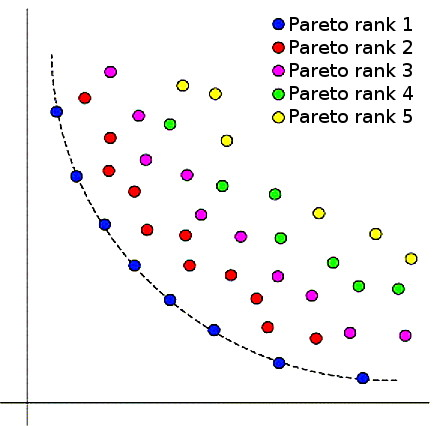
\includegraphics[width=0.6\linewidth]{paretorank}
\end{center}
\caption{Illustration of Pareto ranks}
\label{fig:paretorank}
\end{figure}

\begin{definition}[Crowding distance \cite{Deb00afast}]
The crowding distance is a measure of how close a point is to it neighbours, and thus of the density of solutions surrounding a particular point in the population. It is computed by taking the average distance of the two points on either side of this point along each of the objectives (see. Figure \ref{fig:crowding_dist} and Algorithm \ref{alg:crowding_dist}).
\end{definition}

\begin{figure}[h!]
\begin{center}
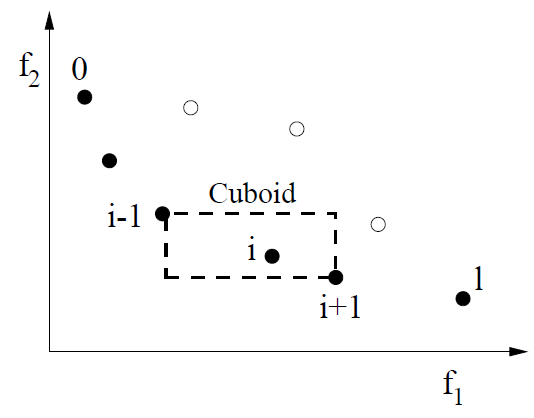
\includegraphics[width=0.6\linewidth]{crowdingdist}
\end{center}
\caption{Crowding distance calculation \cite{Deb00afast}}
\label{fig:crowding_dist}
\end{figure}

\begin{algorithm}[h!]
\caption{Crowding distance for the set of solutions $A$ \cite{Deb00afast}}
\label{alg:crowding_dist}
\KwIn{$A$}
%\SetKwFunction{crowding}{crowding-distance-assignment}
%\crowding{$A$}\\
$l = |A|$;\\
\ForEach{i}{
	set $A[i]_{distance} = 0$;
	}
\ForEach{objective $m$}{
	$A$ = sort($A$,m);\\
	$A[1]_{distance} = A[l]_{distance} = \infty$;\\
	\For{$i = 2$ to $(l-1)$}{
		$A[i]_{distance} = A[i]_{distance} + (A[i+1].m - A[i-1].m)$
		}
	}
\KwSty{Note:} \CommentSty{$A[i].m$ refers to the $m$-th objective function value of the $i$-th individual in the set $A$}
\end{algorithm}

The number of solutions per generation is fixed as constant. Between two solutions with different Pareto ranks, the lower rank will be preferred. Otherwise, if both solutions have the same Pareto rank then the one located in a less-crowded region will be preferred.

\subsubsection{Performance evaluation of a metaheuristic}
In order to evaluate the performance of a metaheuristic, several metrics have been defined in the literature to assess the convergence and diversity properties of an algorithm \cite{talbi09}. Among the classical indicators, one can cite the contribution indicator, the spread indicator, the binary $\epsilon$-indicator, the unary hypervolume indicator and the density of the Pareto-front which are presented in \cite{talbi09, 1197687}. These indicators can be grouped in 3 categories defined in \cite{talbi09}:
\begin{enumerate}
	\item The convergence-based indicators:
	\begin{quote}
		\emph{"The convergence metrics evaluate the effectiveness of the solutions in terms of the closeness to the optimal Pareto front."}
	\end{quote}
	\item The diversity-based indicators:
	\begin{quote}
		\emph{"Diversity indicators measure the uniformity of distribution of the obtained solutions in terms of dispersion and extension. In general, the diversity is researched in the objective space."}
	\end{quote}
	\item The hybrid indicators: that combine both convergence and diversity measures.
\end{enumerate}

% Other convergence-based indicators such as the generational distance, the $\epsilon$-indicator, a cardinality measure and a distance measure cannot currently be applied for our problem since we do not have a reference set to compare to.

\paragraph{Contribution indicator}
%\label{app:cont}
The contribution is a convergence-based binary indicator. The contribution of an approximation $PO_1$ relatively to another approximation $PO_2$ is the ratio of non-dominated solutions produced by $PO_1$ in $PO^*$, which is the set of Pareto solutions of $PO_1 \cup PO_2$ \cite{talbi09}:
\begin{equation}
Cont(PO_1/PO_2) = \frac{\frac{\|PO\|}{2}+\|W_1\|+\|N_1\|}{\|PO^*\|}
\end{equation}
where $PO$ is the set of solutions in $PO_1 \cap PO_2$, $W_1$ the set of solutions in $PO_1$ that dominate some solutions of $PO_2$ and $N_1$ the set of non-comparable solutions of $PO_1$. This value has to be greater than 0.5 to indicate that $PO_1$ is better than $PO_2$ in terms of convergence to the Pareto front.

\paragraph{Spread indicator}
%\label{app:spread}

The spread indicator $I_s$ combines the distribution and cardinality to measure the dispersion of the approximated Pareto set $A$ \cite{talbi09}:
\begin{equation}
I_s = \frac{\sum_{u \in A}|\{u' \in A: \|F(u)-F(u')\|>\sigma\}|}{|A|-1}
\end{equation}
where $F(u)$ is a fitness function and $\sigma > 0$ a neighborhood parameter. The closer is the measure to 1, the better is the spread of the approximated set $A$.

\paragraph{Binary $\epsilon$-indicator}
The binary $\epsilon$-indicator is a convergence-based indicator. It will give the quality of a solution front in comparison with a another set, with regards to all objectives. Let us consider a minimization problem with $n$ positive objectives. An objective vector $f^1 = (z_1^1, z_2^1, \dots, z_n^1)$ is said to $\epsilon$-dominate another objective vector $f^2 = (z_1^2, z_2^2, \dots, z_n^2)$ if $\forall 1 \leq i \leq n : \: z_i^1 \leq \epsilon \cdot z_i^2$, for a given $\epsilon > 0$. A binary $\epsilon$-indicator $I_\epsilon(A,B)$ gives the factor $\epsilon$ such that for any solution in $B$ there is at least one solution in $A$ that is not worse by a factor of $\epsilon$ in all objectives. $I_\epsilon(A,B)$ can be calculated as follows \cite{1197687}:
\begin{equation}
I_\epsilon(A,B) = \max\limits_{z^2 \in B} \: \min_{z^1 \in A} \: \max_{1 \leq i \leq n} \: \frac{z_i^1}{z_i^2}
\end{equation}

\paragraph{Unary hypervolume indicator}
The hypervolume is an hybrid indicator. Since we already cited a binary indicator (\textit{epsilon}), we will define the hypervolume indicator $I_H$ in its unary form. $I_H$, associated with an approximation set $A$ is given by the volume of the space portion that is weakly dominated by the set $A$ \cite{talbi09}.

\subsection{Multi-criteria decision aid}
\label{subsec:mcda}
Once the Pareto frontier is obtained or approximated, the compromise solutions can be found by establishing a preference model of the decision maker facing several conflicting solutions. Those models can be classified into three broad categories \cite{Vin92, beltstew} whose methods will be detailed in Section \ref{subsec:mcdamethods}:

\begin{enumerate}
\item \textit{Aggregation methods}: numerical scores are calculated by aggregating the criteria to determine the level of preference for a solution. The most known aggregation methods are the Multi-Attribute Utility Theory (MAUT) \cite{MMAUT} and the Analytic Hierarchy Process \cite{MAHP}.
\item \textit{Interactive methods}: it is a sequential process composed by alternating computation steps and dialogue with the decision maker. A first compromise is submitted to the decision maker who can accept or deny it. If the solution is denied, the DM can give extra information (e.g. releasing a constraint) about his preferences (dialogue) and a new solution can be calculated, so a new decision process begins. Otherwise, no better solution can be found and the process stops. Among the most known interactive methods, the STEP Method (STEM) \cite{benayoun71} or the Satisficing Trade-Off Method (STOM) \cite{nakayama84} can be cited.
\item \textit{Outranking methods}: the solutions are compared pairwise which enables the possibility to identify the relationship between the solutions. This shows the preference for a solution in comparison to another one. PROMETHEE \cite{Brans1} and ELECTRE \cite{Roy66} are among the most known outranking methods.
\end{enumerate}

%Those methods will not be described further here, as they can be found in reference books such as \cite{Vin92}, \cite{BraMar2002, EhrgottFigueiraGreco2005, beltstew, Sch85}.

Generally, the purpose of MCDA is to provide answers for three main problematic \cite{EhrgottFigueiraGreco2005}:
\begin{enumerate}
\item \textit{The choice problematic (P.$\alpha$)}: the aid aims the selection of a small number of good solutions in such way that one or several compromise solutions can be chosen.
\begin{example}
In circuit design, the objective would be to choose the best compromise CPU in terms of performance and price.
\end{example}
\item \textit{The sorting problematic (P.$\beta$)}: the aid aims the assignment of each solution to a predefined (ordered) category.
\begin{example}
%Usage pro, casual, gamer
Depending on performance, price, radiation resistance, thermal operational range, electronic components can be sorted following robustness constraints for commercial, industrial or military and spatial purposes
\end{example}
\item \textit{The ranking problematic (P.$\gamma$)}: the aid aims the complete or partial preorder of all the solutions.
\begin{example}
With a preorder for CPUs based on an assessment of their performance, it is possible to associate a price to each processor depending on their ranking.
\end{example}
\end{enumerate}

\subsection{Preference modelling}
\label{sec:prefmod}
As mentioned, preference modelling is an important step in decision making problem. It is necessary to understand how a model is built as it will determine how a method will work based on it and thus the outcoming results.

\subsubsection{Definitions}
Before introducing some important MCDA methods, let us first define some definitions about preference modelling in order to ease the understanding of the following sections.

When modelling the decision maker's preferences, three binary relations which result from the comparison of two alternatives $a_i$ and $a_j \in \mathcal{A}$ are defined \cite{Vin92}:
\begin{equation}
\left\{
\begin{array}{ll}
a_iPa_j & \text{ if $a_i$ is prefered to $a_j$}\\
a_iIa_j & \text{ if $a_i$ is indifferent to $a_j$}\\
a_iRa_j & \text{ if $a_i$ is incomparable to $a_j$}\\
\end{array}
\right.
\end{equation}

These relations express situations of preference, indifference and incomparability and it can be assumed that they satisfy the following properties:

\begin{equation}
\forall a_i, a_j \in \mathcal{A} \left\{
	\begin{array}{ll}
	a_iPa_j \Rightarrow a_i \neg P a_j : & \text{: $P$ is asymmetric}\\
	a_iIa_i & \text{: $I$ is reflexive}\\
	a_iIa_j \Rightarrow a_jIa_i & \text{: $I$ is symmetric}\\
	a_i \neg R a_i & \text{: $R$ is irreflexive}\\
	a_iRa_j \Rightarrow a_jRa_i & \text{: $R$ is symmetric}
	\end{array}
\right.
\end{equation}

Intuitively:
\begin{itemize}
\item aPb corresponds to the existence of clear and positive reasons that justify significant preference in favour of a
\item aIb corresponds to the existence of clear and positive reasons that justify equivalence between the two alternatives
\item aRb corresponds to an absence of clear and positive reasons that justify any of the two preceding relations
\end{itemize}

As stated, $(P,I,R)$ are binary relations. However, these relations can be poor in terms of information about the preferences of a decision maker. Indeed, $P$ will for instance express a strict preference between two alternatives whereas the DM can have a degree of intensity of the preference. For such kinds of situations, the preferences can be defined by a valued preference relation. This valued relation will often take values in the interval $[0; 1]$ \cite{EhrgottFigueiraGreco2005}.

\subsection{Some important multi-criteria methods}
\label{subsec:mcdamethods}

\subsubsection{Multi-Attribute Utility Theory}
Multi-Attribute Utility Theory (MAUT) has been introduced by Fishburn \cite{Fishburn70} and Keeney and Raiffa \cite{KeeneyRaiffa76}. This method belongs to the family of aggregation methods that consist in substituting the initial multi-criteria problem
\begin{equation}
\min \{f_1(x), f_2(x), \dots, f_m(x) | x \in \mathcal{A}\}
\end{equation}
the following uni-criterion problem:
\begin{equation}
min \{U(x) | x \in \mathcal{A}\}
\end{equation}
where $U(x)$ is called the utility function that aggregates all the criteria to a single criterion:
\begin{equation}
U(x) = U[f_1(x), f_2(x), \dots, f_m(x)]
\end{equation}

Generally, this utility function is a non-linear function defined such that:
\begin{eqnarray}
U(a) > U(b) &\Leftrightarrow& a \text{ is prefered to } b\\
U(a) = U(b) &\Leftrightarrow& a \text{ is indifferent to } b
\end{eqnarray}

One of the most used utility function is the weighted sum:
\begin{equation}
U(x) = \sum_{j=1}^{m} w_j f_j(x)
\end{equation}
where $w_j$ is the weight associated to the criterion $j$.

With this utility function, it is then possible to compute an aggregated score for each solutions and rank them in order to choose among the best ones.

MAUT has been applied in numerous cases and developments have been provided to axiomatize this method and justify its use \cite{MMAUT}.

\subsubsection{Analytical Hierarchy Process (AHP)}
Analytical Hierarchy Process (AHP) has been developed by Saaty \cite{MAHP}. This multi-criteria method allows to face structurally complex choices by decomposing the problem in several sub-problems that can be analysed independently and are easier to understand. Similarly to PROMETHEE and ELECTRE, AHP proceeds by making pairwise comparisons of the alternatives, but for example on basis of a ordinal scale from 1 to 9. Indeed, one of the distinctive features of this methods is to build a matrix by asking the decision maker to compare all pairs of alternatives and criteria. Therefore, the input for AHP is not an evaluation table but the DM's preference matrix. The normalized right-hand eigenvector of this matrix is then used to compute the score associated to each alternative and the weight associated to each criterion. 

In order to illustrate AHP, we will give more details on a particular case where only the criteria are compared. The decision maker will make pairwise comparisons and give an ordinal scale of preference for the criteria. The following matrix can be obtained:
\begin{equation}
A=\begin{pmatrix}
1 & a_{12} & \dots & a_{1j} & \dots & a_{1m}\\
\frac{1}{a_{12}} & 1 & \dots & a{2j} & \dots & a_{2m}\\
\vdots \\
\frac{1}{a_{1j}} & \frac{1}{a_{2j}} & \dots & a_{ij} & \dots & a_{im}\\
\vdots \\
\frac{1}{a_{1m}} & \frac{1}{a_{2m}} & \dots & a_{im} & \dots & 1
\end{pmatrix}
\end{equation}
where $a_{ij}$ is expresses the relative importance of the criterion $i$ over the criterion $j$.

From this matrix, AHP uses a method based on eigenvector to extract the related weights of each criterion that can be used, for instance, as input data for MAUT in a weighted sum.

A comparison matrix is said to be consistent if $a_{ij} a_{jk} = a_{ik} \forall i, j, k$. However, consistency cannot always be reached and AHP's developers have defined a Consistency Index (CI):
\begin{equation}
CI = \frac{\lambda_{max}-m}{m-1}
\end{equation}
where $\lambda_{max}$ is the largest eigenvalue of the matrix and $m$ is the matrix size.

This Consistency Index is then compared to Random (consistency) Index (RI) which are considered to be appropriate CIs. These RIs are obtained by randomly generating matrices and taking the average CI values.

A Consistency Ratio (CR) then is defined:
\begin{equation}
CR = \frac{CI}{RI}
\end{equation}
If the value of the Consistency Ratio is lower or equal to 10\%, the inconsistency is considered to be acceptable. Otherwise, the decision maker has to revise judgements.

%This methods can be summarized in seven key steps \cite{Vaidya20061}
%\begin{enumerate}
%\item State the problem
%\item Broaden the objectives of the problem or consider all actors, objectives and its outcome.
%\item Identify the criteria that influence the behaviour.
%\item Structure the problem in a hierarchy of different levels constituting goal, criteria, sub-criteria and alternatives.
%\item Compare each element in the corresponding level and calibrate them on the numerical scale. Consequently build the comparison matrix with the computed valued based on the comparisons.
%\item Compute the highest eigenvalue of the matrix, the consistecy index (CI), the consistency ration (CR) and the normalized values for each criterion/alternative.
%\item If the maximum eigenvalue, CI and CR are satisfactory, the decision is taken based on the normalized values. Otherwise, the procedure is repeated until these values reach an acceptable range.
%\end{enumerate}

\subsubsection{STEP Method (STEM)}
The STEP Method has been proposed by Benayoun \cite{benayoun71}. STEM is an interactive and iterative exploration procedure that aims to reach the best compromise according the decision maker after a certain number of cycles. Each cycle is composed of a calculation phase and a decision-making phase (discussion with the decision maker):
\begin{enumerate}
\item An efficient compromise solution is determined.
\item \label{stem2} This solution is submitted to the decision maker. Three cases can then happen:
	\begin{enumerate}
	\item The decision maker is satisfied and the procedure ends;
	\item The decision maker wants to simultaneously improve all the evaluations. This is impossible since the proposed solution is efficient. The procedure ends and cannot help the decision maker.
	\item The decision maker identifies a particular criterion on which a concession can be made in order to improve other criteria. A new efficient solution can then be determined.
	\item This new solution is submitted. Go to step \ref{stem2}.
	\end{enumerate}
\end{enumerate}

\subsubsection{Satisficing Trade-Off Method (STOM)}
The STOM method has been proposed by Nakayama \cite{nakayama84}. Similarly to STEM, it relies on a discussion with the decision maker but is based on the setting of an ideal point defined as follows:
\begin{definition}[Ideal point]
The ideal point $f^*=(f_1^*, f_2^*, \dots, f_m^*)$ is defined such that $f_i^* = \min \{f_i(x), \forall i=1, 2, \dots, m, \forall x \in \mathcal{A}\}$.
\end{definition}
The ideal point possesses as coordinates the best values that can be achieved for each criterion separately.

STOM can be summarized in four steps:
\begin{enumerate}
\item The first step is to set the ideal point.
\item Then the aspiration level for each criterion is asked to the decision maker; this is the reference point for each criterion of the decision maker. Note that the aspiration level should be lower than the ideal point.
\item \label{stom3} A Pareto solution nearest to the ideal point and in the direction of the aspiration level is determined.
\item This solution is submitted to the decision maker. If it is satisfactory, the procedure ends. Otherwise, the decision maker is asked to trade off to define another aspiration level. Go to step \ref{stom3}.
\end{enumerate}

\subsubsection{The PROMETHEE methods}
PROMETHEE (Preference Ranking Organisation METHod for Enrichment Evaluations) has been initiated by Brans \cite{Brans1} and developed with Mareschal \cite{mares2ejor88} and Vincke \cite{BransMarechalVincke84}. In this section, we will only describe the basics of PROMETHEE. More details can be found in \cite{Beh2010}.\\
The PROMETHEE methods are based on the three following steps:
\begin{itemize}
\item Enriching the preference structure: a preference function is introduced to characterize a valued relation (see Section \ref{sec:prefmod})
\item Enriching the dominance relation: a valued outranking relation is determined
\item Decision aid: the valued outranking relations are exploited
\end{itemize}

\begin{enumerate}
\item \textit{\underline{Preference function}}\\
Since the dominance relation is really poor (binary relation), a preference function $P_k(a_i,a_j)$ will be introduce to enrich it. This function gives the preference degree of an alternative $a_i$ over an alternative $a_j$ with respect to the function $d_k(a_i,a_j) = f_k(a_i) - f_k(a_j)$ which is the difference between the evaluation of $a_i$ and $a_j$ for the criterion $k$, assuming a non decreasing function. Of course, this difference of evaluations has to respect some hypothesis such as having the same interval scale.\\
Consequently, it is therefore possible to define several types of preference functions based on preference ($P$) or indifference ($Q$) thresholds, as shown in Table \ref{tab:pref_func}. Below the indifference threshold, the decision maker will consider having no preference while above the preference threshold, the decision maker will have a strict preference.

\begin{table}[h!]
\caption{Preference functions (reproduced from \cite{BraMar2002})}
\begin{center}
\begin{tabular}{|l|c|b{4.2cm}|}
\hline Usual & 
\includegraphics[page=2,trim=7.5cm 13.8cm 3.5cm 6.5cm,clip,scale=0.36]{prom_usual_pdf} & Strict preference\\
\hline U-shape & 
\includegraphics[page=2,trim=7.5cm 13.8cm 3.5cm 6.5cm,clip,scale=0.36]{prom_ushape_pdf} & Q: indifference threshold\\
\hline V-shape & 
\includegraphics[page=2,trim=7.5cm 13.8cm 3.5cm 6.5cm,clip,scale=0.36]{prom_vshape_pdf} & P: preference threshold\\
\hline Level & 
\includegraphics[page=2,trim=7.5cm 13.8cm 3.5cm 6.5cm,clip,scale=0.36]{prom_level_pdf} & Q: indifference threshold \newline P: preference threshold\\
\hline Linear & 
\includegraphics[page=2,trim=7.5cm 13.8cm 3.5cm 6.5cm,clip,scale=0.36]{prom_linear_pdf} & Q: indifference threshold \newline P: preference threshold\\
\hline Gaussian & 
\includegraphics[page=2,trim=7.5cm 13.8cm 3.5cm 6.5cm,clip,scale=0.36]{prom_gaussian_pdf} & S: preference threshold\\
\hline
\end{tabular}
\end{center}
\label{tab:pref_func}
\end{table}

\item \textit{\underline{Valued outranking relation}}\\
\textit{Multi-criteria preference index}

The multi-criteria preference index is defined as follows:
\begin{equation}
\pi (a_i, a_j) = \sum_{k=1}^{m} P_{k}(a_i, a_j).w_{k}, \forall i \neq j \text{ with $\sum_{k=1}^{k} w_{k} = 1$}
\end{equation}
where $w_{k}>0, k=1, 2, ..., m$ are the weights on each criterion. $\pi (a_i, a_j)$ represents a measure of the preference of $a_i$ over $a_j$ on all the criteria.

Let us note the following properties of the preference index:
\begin{eqnarray}
&\pi(a_i,a_i) = 0&\\
&0 \leq \pi(a_i,a_j)&\\
&\pi(a_i, a_j) + \pi(a_j,a_i) \leq 1&
\end{eqnarray}
%\begin{equation}
%\pi(a_i, a_j) + \pi(a_j,a_i)
%\end{equation}

\textit{Outranking flow}

An \og outranking flow \fg is then defined on the basis of the preference index. That allows to compare alternatives with each others. Three types of flow are formulated:
\begin{itemize}
\item The positive outranking flow: $\phi^{+} = \frac{1}{n-1} \sum_{j \neq i} \pi (a_i, a_j)$. This flow expresses how $a_i$ outranks all the other alternatives.
\item The negative outranking flow:$\phi^{-} = \frac{1}{n-1} \sum_{j \neq i} \pi (a_j, a_i)$. This flow expresses how $a_i$ is outranked by all the other alternatives.
\item The net flow: $\phi(a) = \phi^{+}(a_i) - \phi^{-}(a_i)$. This flow expresses the balance between the positive and negative flows of $a_i$
\end{itemize}
Let us note the following properties for these flows:
\begin{eqnarray}
&\phi^{+}, \phi^{-} \in [0;1]&\\
&\phi \in [-1;1]&
\end{eqnarray}

Based on these flows, the PROMETHEE methods will establish an outranking relation.

\item \textit{\underline{PROMETHEE I}}

The positive and negative flows allow to sort the alternatives of $A$. Let $(S^{+}, I^{+})$ and $(S^{-}, I^{-})$ be the two complete pre-orders obtained from these flows:
\begin{equation}
\begin{cases}
a_iS^{+}a_j \Leftrightarrow \phi^{+}(a_i) > \phi^{+}(a_j)\\
a_iI^{+}a_j \Leftrightarrow \phi^{+}(a_i) = \phi^{+}(a_j)
\end{cases}
\end{equation}
This means that the higher the positive flow is, the better the alternative.

\begin{equation}
\begin{cases}
a_iS^{-}a_j \Leftrightarrow \phi^{-}(a_i) < \phi^{-}(a_j)\\
a_iI^{-}a_j \Leftrightarrow \phi^{-}(a_i) = \phi^{-}(a_j)
\end{cases}
\end{equation}
This means that the lower the negative flow is, the better the alternative.

PROMETHEE I establishes a partial ranking by taking the intersection of these two pre-orders:
\begin{equation}
\begin{cases}
a_iP^{(1)}a_j \Leftrightarrow \begin{cases}
	a_iS^{+}a_j \text{ and } a_iS^{-}a_j\\
	a_iS^{+}a_j \text{ and } a_iI^{-}a_j\\
	a_iI^{+}a_j \text{ and } a_iS^{-}a_j
	\end{cases}\\
a_iI^{(1)}a_j \Leftrightarrow a_iI^{+}a_j \text{ and } a_iI^{-}a_j\\
a_iR^{(1)}a_j \text{ otherwise}
\end{cases}
\end{equation}
where $(P^{(1)}, I^{(1)}, R^{(1)})$ represent respectively the preference, the indifference and the incomparability in PROMETHEE I.
\begin{itemize}
\item $a_iP^{(1)}a_j$ (\og $a_i$ is prefered to $a_j$ \fg): $a_i$ is simultaneously better and less worse than $a_j$.
\item $a_iI^{(1)}a_j$ (\og $a_i$ and $a_j$ are indifferent \fg): $a_i$ is neither better nor worse than $a_j$.
\item $a_iR^{(1)}a_j$ (\og $a_i$ and $a_j$ are incomparable \fg): $a_i$ is better than $a_j$ on some criteria while $a_j$ is better than $a_i$ on other criteria.
\end{itemize}

\item \textit{\underline{PROMETHEE II}}

In order to obtain a complete ranking, the net flow will be considered:
\begin{equation}
\begin{cases}
a_iP^{(2)}a_j \Leftrightarrow \phi(a_i) > \phi(a_j)\\
a_iI^{(2)}a_j \Leftrightarrow \phi(a_i) = \phi(a_j)\\
\end{cases}
\end{equation}
where $P^{(2)}$ et $I^{(2)}$ represent respectively the preference and the indifference in PROMETHEE II. This means that the higher the net flow is, the better the alternative.

Let us note that, unlike PROMETHEE I, PROMETHEE II does not give place to incomparability and a complete ranking can directly be obtained.

\item \textit{\underline{The GAIA plane}}

When working with more than three criteria, it is impossible to have a perfect visual representation of the solutions space. The GAIA (Geometrical Analysis for Interactive Assistance) plane can give a visualization even if there are more than three criteria, by means of the principal component analysis (PCA) of the net flows on the decision maker's preferences for each criterion.

The PCA allows a projection of the alternatives on a plane that minimizes the loss of information induced by this projection.

This plan allows to have a visual descriptive analysis with several criteria. It can highlight the conflict and synergy between criteria and show the profiles of the alternatives. This will help to identify the potential compromise solutions.

In order to illustrate the use of the GAIA plane, we will take a simple example: six alternatives evaluated on 5 criteria. The associated GAIA plane is given in Figure \ref{fig:gaiacar}.

\begin{figure}[h!]
\begin{center}
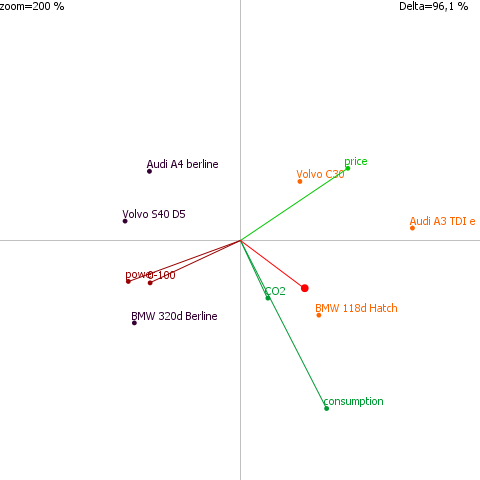
\includegraphics[width=0.8\textwidth]{gaiacar.png}
\end{center}
\caption{Example of a GAIA plane}
\label{fig:gaiacar}
\end{figure}

Four distinctive visual information are shown:
\begin{enumerate}
\item The green axes that represent the projections of each criterion's axis.
\item The blue dots that represent the projection of each solution's uni-criterion net flow. The value of the uni-criterion net flow is read by projecting the point on the related criterion axis.
\item The red axis that represents the \textit{decision axis} which is the projection of the set of weights and gives the decision direction.
\item The \textit{delta} value that represents the percentage of kept information since there are projection errors.
\end{enumerate}

From the GAIA plane, we can observe how the criteria are related between each other. Indeed, criteria axes that have opposite directions are conflicting, whereas criteria with the same direction are in synergy. In this case, we can see that C1 is conflicting with C2 and C3, which is to be expected. Also, C4 and C5a have the same direction.

As for the decision axis, it allows a decision maker to know in which direction the best compromise solutions are located based on the criteria weights. Indeed, the alternatives with the highest net flow score will have their furthest projection on that axis, in the direction of that axis. This visually represents the PROMETHEE II ranking, provided that the \textit{delta} value shows that enough information has been kept with the projection.

\end{enumerate}

\subsubsection{The ELECTRE methods}
ELECTRE (\textit{ELimination Et Choix Traduisant la REalité}, or ELimination and Choice Translating REality) has been developed by Roy \cite{Roy66}. In this section, we will only describe the basics of ELECTRE. More details can be found in \cite{electre}.

\begin{enumerate}
\item \textit{\underline{ELECTRE I}}

ELECTRE I is a method linked to the $P.\alpha$ problematic that aims to obtain a subset $N$ of alternatives such that all the solutions that do not belong to this set are outranked by at least one alternative of $N$ and the solutions of $N$ do not outrank each other. $N$ is therefore not the set of good alternatives but rather the set where the best compromise can certainly be found.

The outranking relation is obtained by establishing a weight $w_k$ for each criterion. A concordance index is the associated to each pair $(a_i, a_j)$ of alternatives:
\begin{equation}
c(a_i, a_j) = \frac{1}{W} \sum_{j:f_{k}(a_i) \leq f_{k}(a_j)}{w_{k}}, \text{ where } W = \sum_{k=1}^{m} w_{k}, w_k > 0
\end{equation}
The concordance index represents a measure of the arguments favourable to the statement \og \textit{$a_i$ outranks $a_j$} \fg.

A discordance index can also be defined:
\begin{equation}
d(a_i, a_j) = \begin{cases}
	0& \text{if $f_{k}(a_i) \geq f_{k}(a_j), \forall k$}\\
	\frac{1}{\delta} \max_{k} [f_{k}(a_j) - f_{k}(a_i)]& \text{otherwise}
	\end{cases}
\end{equation}
The discordance index is therefore higher if the preference of $a_j$ over $a_i$ is strong on at least one criterion.

Then concordance $\hat{c}$ and discordance $\hat{d}$ thresholds are defined alongside the outranking relation $S$:
\begin{equation}
\forall i \neq j, a_iSa_j \text{ iff } \begin{cases}
	c(a_i, a_j) \geq \hat{c}\\
	d(a_i, a_j) \leq \hat{d}
	\end{cases}
\end{equation}

From this definition, a subset $N$ of alternatives (called the kernel) is established such that:
\begin{equation}
\begin {cases}
\forall a_j \in A\setminus N, \exists a_i \in N : a_iSa_j\\
\forall a_i, a_j \in N, a_i \overline{S} a_j
\end{cases}
\end{equation}

A subset $N$ of alternatives is established such that all the alternatives that do not belong to this set is outranked by at least one alternative of $N$ and the alternatives of $N$ are incomparable. The decision process will therefore take place within the set $N$. The kernel exists and is unique when the outranking relation $S$ does not contain circuit in its graph.

\item \textit{\underline{ELECTRE II}}

This method aims to rank the alternatives. The outranking relation is defined by fixing two concordance thresholds $\hat{c}_{1}$ and $\hat{c}_{2}$ such that $\hat{c}_{1} > \hat{c}_{2}$ and by building a strong outranking relation $S^{F}$ and a weak outranking relation $S^{f}$ based on these two thresholds:
\begin{equation}
a_iS^{F}a_j \text{ iff } \begin{cases}
	c(a_i, a_j) \geq \hat{c}_{1}\\
	\sum_{, : f_{k}(a_i)>f_{k}(a_j)} w_{k} > \sum_{k : g_{k}(a)<g_{k}(b)} w_{k}\\
	(f_{k}(a_i), f_{k}(a_j)) \not\in D_{k}, \forall k
	\end{cases}
\end{equation}
\begin{equation}
a_iS^{f}a_j \text{ iff } \begin{cases}
	c(a_i, a_j) \geq \hat{c}_{2}\\
	\sum_{k : f_{k}(a_i)>f_{k}(a_j)} w_{k} > \sum_{k : f_{k}(a_i)<f_{k}(a_j)} w_{k}\\
	(f_{k}(a_i), f_{k}(a_j)) \not\in D_k, \forall k
	\end{cases}
\end{equation}
The discordance can also induce two levels of relations by building two sets of discordance for each criterion.

In order to obtain the ranking, a set is determined from $S^ {F}$. This set $B$ contains the alternatives that are not strongly outranked by any others. From $B$ and $S^{f}$, the set $A^{1}$ of alternatives that are not weakly outranked by any alternatives of $B$ is determined. The set $A^{1}$ constitutes the best alternatives class. $A^{1}$ is then removed and the process is repeated to find $A^{2}$ and so on until a complete pre-order is obtained.

Let us note that a second complete pre-order can be obtained by applying the process first with the less good alternatives class and then the best ones.

\item \textit{\underline{ELECTRE III}}

This method takes into account the indifference and preference thresholds. It is based on a valued outranking relation that is less sensible to data and parameters variabilities.% but at the cost of arbitrary choice for threshold functions values and an increased complexity for the decision maker.

In ELECTRE III, an outranking degree $S(a_i, a_j)$ associated to each pair $(a_i, a_j)$ of alternatives is defined. It can be understood as an \og degree of credibility of outranking \fg of $a_i$ over $a_j$.

A weight $w_{k}$ is associated to each criterion and for each pair $(a_i, a_j)$ of alternatives the concordance index is computed as follows:
\begin{equation}
c(a_i, a_j) = \frac{1}{W} \sum_{k=1}^{m} w_{k} c_{k}(a_i, a_j), \text{ where } W = \sum_{k=1}^{m} w_{k}
\end{equation}
with
\begin{equation}
c_{k}(a_i,a_j) = \begin{cases}
	1& \text{if } f_{k}(a_i)+q_{k}(f_{k}(a_i)) \geq f_{k}(a_j)\\
	0& \text{if } f_{k}(a_i)+p_{k}(f_{k}(a_i)) \leq f_{k}(a_j)\\
	\text{linear}& \text{if } \begin{array}{rr} f_{k}(a_i)+q_{k}(f_{k}(a_i)) \leq f_{k}(a_j)\\
	\leq f_{k}(a_i)+p_{k}(f_{k}(a_i)) \end{array}
	\end{cases}
\end{equation}
where $q_{k}$ et $p_{k}$ represent respectively the indifference and preference thresholds.

The definition of discordance is then enriched by the introduction of a veto threshold $v_k(f_k(a_i))$ for each criterion $k$ such that any credibility for the outranking of $a_j$ by $a_i$ is refused if $f_k(a_j) \geq f_k(a_i) + v_k(f_k(a_i))$.

A discordance index is then defined:
\begin{equation}
D_k(a_i, a_j) = \begin{cases}
	0 & \text{if } f_k(a_j) \leq f_k(a_i) + p_k(f_k(a_i))\\
	1 & \text{if } f_k(a_j) \geq f_k(a_i) + v_k(f_k(a_i))\\
	\text{linear} & \text{if } \begin{array}{rr} f_k(a_i) + p_k(f_k(a_i)) \leq f_k(a_j)\\
	\leq f_k(a_i) + v_k(f_k(a_i)) \end{array}
	\end{cases}
\end{equation}

The degree of outranking is finally defined:
\begin{equation}
S(a_i,a_j) = \begin{cases}
	c(a_i,a_j) & \text{if } \begin{array}{rr}D_k(a_i,a_j) \leq c(a_i,a_j)\\
		\forall k \end{array}\\
	c(a_i,a_j) \prod_{k \in \mathcal{F}(a_i,a_j)} \frac{1-D_k(a_i,a_j)}{1-c(a_i,a_j)} & \text{otherwise}
	\end{cases}
\end{equation}
where $\mathcal{F}(a_i,a_j)$ is the set of criteria for which $D_k(a_i,a_j) > c(a_i,a_j)$. The degree of outranking is thus equal to the concordance index when no criterion is discordant, otherwise the concordance index is decreased proportionally depending on the importance of the discordances.

A value $\lambda = \max_{a_i,a_j \in \mathcal{A}, i \neq j} S(a_i, a_j)$ is determined and only the outranking degree that have a value greater or equal to $\lambda - s(\lambda)$, where $s(\lambda)$ is a threshold to be determined, are considered. A ranking can then be determined from a qualification index $Q(a)$ for each alternative $a$ that represents the difference between the number of outranked alternatives by $a$ and the number of alternatives that outrank $a$. The set of actions having the largest qualification will be called the first distillate $D_1$.

If $D_1$ contains only one alternative, the previous procedure is repeated with $A \setminus D_1$. Otherwise the same procedure is applied for $D_1$ and if the obtained distillate $D_2$ contains only one alternative, the procedure is repeated with $D_1 \setminus D_2$. Otherwise, it is applied for $D_2$, and so on until $D_1$ is completely used, before starting with $A \setminus D_1$. This procedure produces a first complete preorder.

A second complete preorder can be obtained by applying the opposite procedure where the alternatives with the smallest qualification are first used.

%\item \textit{\underline{ELECTRE IV}}
%
%This method is similar to ELECTRE III and aims to sort alternatives but without considering weights on the criteria.
\end{enumerate}

\section{Conclusion}
In this chapter, we have given a short overview of multi-objective optimization and multi-criteria decision aid. We have explained in what kind of context a multi-criteria paradigm can be applied and have presented some of the classical method used in the field.

In the next chapter, we will define the problem we tackle and show how a 3D-SIC can be modelled in order to apply multi-objective optimization.